\chapter{Physics behind numerical methods}\label{Formulae}

\section{Distribution function transform}
Distribution function of particles in phase space is presented in code in spherical coordinates $n(\epsilon,\mu,\phi)$. Let consider transform to the frame moving along $z$-axis with lorentz-factor $\gamma = 1/\sqrt{1-\beta^2}$. Number of particles in the corresponding phase volumes $N$ is invariant.

\begin{equation}
	N = n(\epsilon,\mu,\phi)d\epsilon d\mu d\phi dV = n'(\epsilon',\mu',\phi')d\epsilon' d\mu' d\phi' dV'
\end{equation}

So, to obtain $n'$ we need to evaluate determinant of Jacobi transformation matrix. Note, that azimuthal angle phi does not changes in transformation to the moving frame $phi' = phi$, and energy and polar angle does not depend on space volume, so in general Jacobi matrix has following non-zero terms

\begin{equation}\label{generalJacobi}
	J=\left(
	\begin{array}{cccc}
		\frac{d\epsilon'}{d\epsilon} & \frac{d\epsilon'}{d\mu}& 0 & 0\\
		\frac{d\mu'}{d\epsilon} & \frac{d\mu'}{d\mu} & 0 & 0\\
		0 & 0 & 1 & 0\\
		\frac{dV'}{d\epsilon} & \frac{dV'}{d\mu} & 0 & \frac{dV'}{dV}
	\end{array}
	\right)
\end{equation}

Note, that determinant of this matrix can be decomposed by the last column and we get

\begin{eqnarray}
|J|=\frac{dV'}{dV}\left(\frac{d\epsilon'}{d\epsilon}\frac{d\mu'}{d\mu} - \frac{d\epsilon'}{d\mu}\frac{d\mu'}{d\epsilon}\right)
\end{eqnarray}

Let start with transforming space volume $V$. First approach, following Landau-Lifshitz 2, paragraph 10 \cite{LandauLifshitz2}, is to transform volume to the rest-frame of moving beam of particle with given momentum, and then derive that $dV'/dV= \epsilon/\epsilon'$. It is correct result, but proof is not valid for massles particles, which have not physical rest frame.

So we evaluate transformation of volume, containing chosen particles, directly from Lorentz transformations. Let assume flux of particles, aligned with z axis, with uniform interval $L$ between them, moving with same velocity $v$ with angle $\theta$ to the z axis, and $\mu = cos(\theta)$, as it is shown in Figure \ref{VolumeTransform}.

\begin{figure}[h]
	\centering
	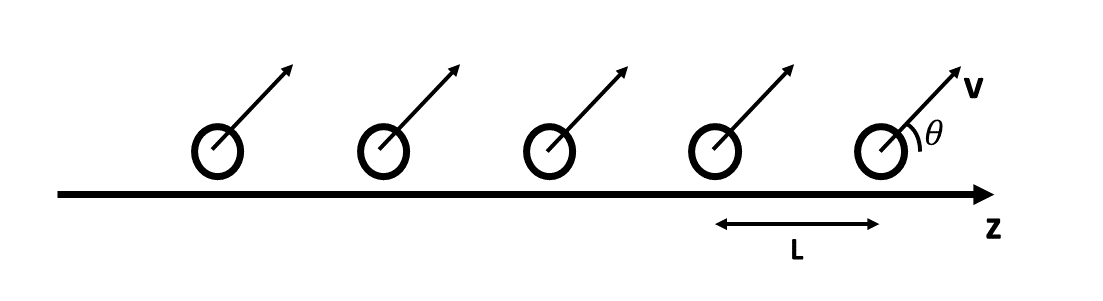
\includegraphics[width=12.5 cm]{./fig/VolumeTransform.png} 
	\caption{Beam of evenly distributed particles}
	\label{VolumeTransform}
\end{figure}

So in the lab frame, at the moment $t$ i-th particle is placed at $z_i = i\cdot L + \mu v t$. Let evaluate coordinates of particles in the moving frame.

\begin{equation}\label{lorentz_z}
	\left(\begin{array}{c}
		ct'\\
		z'_i
	\end{array}
	\right)
	= \left(
	\begin{array}{cc}
		\gamma & -\beta\gamma\\
		-\beta\gamma & \gamma
	\end{array}
	\right)
	\times
	\left(\begin{array}{c}
		ct\\
		z_i
	\end{array}
	\right)
\end{equation}

From this we can obtain values $z'_i = \gamma z_i + (\gamma \mu v - c\beta \gamma)t$, but this values are measured at the different time moments in the moving frame, if $t$ is the same for all particles in lab frame. To evaluate volume or number density we should evaluate them at the same moment $t'$. So let express $t$ in terms of $z_i$ and $t'$, and put into the equation for $z'_i$.

\begin{equation}
	t=\frac{t'+\gamma\beta z_i/c}{\gamma - \beta \mu v/c}
\end{equation}

and

\begin{equation}
	z'_i=\gamma z_i +(\gamma \mu v - c\beta \gamma)\frac{t'+\gamma\beta z_i/c}{\gamma - \beta \mu v/c}=z_i\frac{1}{\gamma(1-\beta\mu v/c)} + t'\frac{\mu v/c - \beta}{1 - \beta \mu v/c}
\end{equation}

Second term, containing $t'$ gives us standard  relativistic velocity-addition formula. And the first one gives a desired expression to the compression of the distance between particles. $L' = z'_{i+1}-z'_i = L/(\gamma(1-\beta\mu v/c))$. The distances in the transversal directions does not comress with Lorentz transformations, so volume also transforms as
\begin{equation} \label{volume}
V' = V/(\gamma(1-\beta\mu v/c))
\end{equation}
This result is the same, as given by \cite{LandauLifshitz2}.

Next, we need to find expressions for $\epsilon'$ and $\mu'$, but it is better to deal with them in to separate cases - for massless and massive particles.

\subsection{Photons}
For massles photons, we consider transformation of energy-mometum vector, taking into account that $z$ component of momentum is $p_z = \mu \epsilon/c$, and transversal components stay constant.

\begin{equation}\label{lorentz_ph}
	\left(\begin{array}{c}
		\epsilon'\\
		\mu'\epsilon'
	\end{array}
	\right)
	= \left(
	\begin{array}{cc}
		\gamma & -\beta\gamma\\
		-\beta\gamma & \gamma
	\end{array}
	\right)
	\times
	\left(\begin{array}{c}
		\epsilon\\
		\mu\epsilon
	\end{array}
	\right)
\end{equation}

From the first line we get equation for Doppler shift of photon's energy

\begin{equation}\label{doppler_ph}
	\epsilon'=\gamma(1-\mu\beta)\epsilon
\end{equation}

Derivatives of $\epsilon'$ with respect to $\epsilon$ and $\mu$ are

\begin{equation}
	\frac{d\epsilon'}{d\epsilon}=\gamma(1-\mu\beta)
\end{equation}

\begin{equation}
	\frac{d\epsilon'}{d\mu}=-\gamma\beta\epsilon
\end{equation}

From the second line of \ref{lorentz_ph} we get
 $\mu'\epsilon'=-\beta\gamma\epsilon+\gamma\mu\epsilon$. Then we plug in expression for $\epsilon'$ from \ref{doppler_ph} and obtain equation for aberration of light
 
\begin{equation}\label{aberration_ph}
	\mu'=\frac{\mu-\beta}{1-\mu\beta}
\end{equation}

Angle of photon's velocity to the z-axis does not depend on their energy. And derivative of $\mu'$ with respect to $\mu$ is

\begin{equation}
	\frac{d\mu'}{d\mu} = \frac{d\mu'}{d\mu}=\frac{d}{d\mu}\frac{1}{\beta}\frac{\beta\mu-1+1-\beta^2}{1-\mu\beta}=\frac{d}{d\mu}\frac{1}{\beta}\frac{1-\beta^2}{1-\mu\beta}=\frac{1-\beta^2}{(1-\mu\beta)^2}=\frac{1}{\gamma^2(1-\mu\beta)^2}
\end{equation}

And Jacobi matrix of coordinate transformation in case of photons is
\begin{equation}
	J=\left(
	\begin{array}{cccc}
		\frac{d\epsilon'}{d\epsilon} & \frac{d\epsilon'}{d\mu}& 0 & 0\\
		0 & \frac{d\mu'}{d\mu} & 0 & 0\\
		0 & 0 & 1 & 0\\
		0 & \frac{dV'}{d\mu} & 0 & \frac{dV'}{dV}
	\end{array}
	\right)
\end{equation}

Determinant of thos matrix, fortunately, equals to the multiple of diagonal terms

\begin{equation}\label{jacobian_ph}
	\frac{D(\epsilon',\mu',\phi',V')}{D(\epsilon,\mu,\phi,V)}=\frac{d\epsilon'}{d\epsilon}\frac{d\mu'}{d\mu}\frac{dV'}{dV}=\gamma(1-\mu\beta)\frac{1}{\gamma^2(1-\mu\beta)^2}\frac{1}{\gamma(1-\mu\beta)}=\frac{1}{\gamma^2(1-\mu\beta)^2}
\end{equation}

And finally, photons distribution function in spherical coordinates transforms as
\begin{equation}\label{distribution_ph}
	n'_{ph}(\epsilon',\mu',\phi') = \frac{n_{ph}(\epsilon,\mu,\phi)}{\frac{D(\epsilon',\mu',\phi',V')}{D(\epsilon,\mu,\phi,V)}}=\gamma^2(1-\mu\beta)^2 n_{ph}(\epsilon,\mu,\phi)
\end{equation}
\subsection{Massive particles}
In the case of massive particles, expression for $\epsilon'$ and $\mu'$ are more complicated. Now $p_z = \mu \sqrt{\epsilon^2 - m^2 c^4}/c$, where $m$ is particle mass, and Lorentz transformation of energy-momentum vector is expressed as

\begin{equation}\label{lorentz_m}
	\left(\begin{array}{c}
		\epsilon'\\
		\mu'\sqrt{{\epsilon'}^2 - m^2 c^4}
	\end{array}
	\right)
	= \left(
	\begin{array}{cc}
		\gamma & -\beta\gamma\\
		-\beta\gamma & \gamma
	\end{array}
	\right)
	\times
	\left(\begin{array}{c}
		\epsilon\\
		\mu\sqrt{{\epsilon}^2-m^2 c^4}
	\end{array}
	\right)
\end{equation}

So expressions for $\epsilon'$ and $\mu'$ are

\begin{equation}
	\epsilon' = \gamma\epsilon-\beta\gamma\mu\sqrt{\epsilon^2-m^2 c^4}
\end{equation}
\begin{equation}
	\mu' = \frac{-\beta\gamma\epsilon+\gamma\mu\sqrt{{\epsilon}^2-m^2 c^4}}{\sqrt{{\epsilon^2 - m^2 c^4}}}
\end{equation}

And expresson for volume transformation \ref{volume} in terms of $\epsilon$ and $\mu$ is
\begin{equation}
	V'=\frac{V}{\gamma(1-\mu\beta\sqrt{{\epsilon}^2-m^2 c^4}/\epsilon)}
\end{equation}

Expressions for partial derivatives of $\epsilon'$, $\mu'$, $V'$, and especially for Jacobian are really terrible, so here we present only final result for distribution function in units $c = 1$

\begin{equation}
		\frac{n'_{m}(\epsilon',\mu',\phi')}{n_{m}(\epsilon,\mu,\phi)}= \frac{\gamma(\epsilon-\mu\sqrt{{\epsilon}^2-m^2}\beta)(\gamma^2\epsilon^2-m^2 + \mu^2 ((\epsilon^2-m^2)(\gamma^2-1)) - 2\mu\epsilon\gamma^2\beta\sqrt{\epsilon^2-m^2})^{3/2}}{\epsilon(((\gamma^2-1)(\epsilon^2-m^2)\mu^2 + \gamma^2\epsilon^2 - m^2)\sqrt{\epsilon^2-m^2}-2\mu\epsilon\gamma(\epsilon^2 - m^2)\sqrt{\gamma^2 - 1})}
\end{equation}

\section{Inverse Compton scattering}\label{comptonFormulaSection}

Consider scattering of photons on the one electron, moving along z axis, following \cite{Dubus}. Klein-Nishina cross-section in electron's rest frame is

\begin{equation}\label{KleinNishina}
	\frac{d\sigma}{d\epsilon_1'd\Omega_1'}=\frac{{r_e}^2}{2}\left(\frac{\epsilon_1'}{\epsilon_0'}\right)^2\left(\frac{\epsilon_1'}{\epsilon_0'}+\frac{\epsilon_0'}{\epsilon_1'}-\sin^2\Theta'\right) \delta\left(\epsilon_1' - \frac{\epsilon_0'}{1+\frac{\epsilon_0'}{m_e c^2}(1 - \cos \Theta')}\right)
\end{equation}

Where $r_e$ - classical electron radius, $\epsilon_0'$ and $\epsilon_1'$ - photon initial and final energies respectively $\Theta'$ angle between initial and final photon directions, defined by expression $\cos\Theta' =\cos \theta_0' \cos \theta_1' + \sin \theta_0' \sin \theta_1' \cos(\phi_1' - \phi_0')$. Primed values are measured in the electron's rest frame. Final and initial photon's energies are related as follow:

\begin{equation}
	\epsilon_1'=\frac{\epsilon_0'}{1+\frac{\epsilon_0'}{m_e c^2}(1 - \cos \Theta')}	
\end{equation}

\begin{equation}
	\epsilon_0'=\frac{\epsilon_1'}{1-\frac{\epsilon_1'}{m_e c^2}(1 - \cos \Theta')}
\end{equation}

Number of photons, which are scattered in unit solid angle in unit energy range in time unit in electron's rest frame is 

\begin{equation}
\frac{dN'}{dt'd\epsilon_1'd\Omega_1'}=\int c \frac{d\sigma}{d\epsilon_1'd\Omega_1'} \frac{dn'}{d\epsilon_0'd\Omega_0'}d\Omega_0'd\epsilon_0'
\end{equation}

Let rewrite delta-function in \ref{KleinNishina} with photon initial energy using relation

\begin{equation}
	\delta(f(x)) = \sum \frac{\delta(x-x_k)}{|f'(x_k)|}
\end{equation}

where $x_k$ - are roots of $f(x)$. Derivative of expression inside delta-function is

\begin{equation}
	\frac{d\epsilon_1'}{d\epsilon_0'}=\frac{1}{(1+\frac{\epsilon_0'}{m_e c^2}(1 - \cos \Theta'))^2}
\end{equation}

and it will cancel out with $\left(\epsilon'_1/\epsilon'_0\right)^2$ in \ref{KleinNishina}. Initial photons distribution function in the lab frame is $\frac{dn}{d \epsilon_0 d \Omega_0}$, and we transform it to the electron frame using \ref{distribution_ph}.

\begin{equation}
	\frac{dN'}{dt'd\epsilon_1'd\Omega_1'}=\int \frac{r_e^2 c}{2} \gamma_e^2 (1 - \mu_0 \beta_e)^2 \left(\frac{\epsilon_1'}{\epsilon_0'}+\frac{\epsilon_0'}{\epsilon_1'}-\sin^2\Theta'\right)\frac{dn}{d\epsilon_0 d\Omega_0} \delta\left(\epsilon_0' - \frac{\epsilon_1'}{1-\frac{\epsilon_1'}{m_e c^2}(1 - \cos \Theta')}\right) d\epsilon_0'd\mu_0' d\phi_0'
\end{equation}

Now we get rid of delta-function by integrating over $\epsilon_0'$

\begin{equation}
	\frac{dN'}{dt'd\epsilon_1'd\Omega_1'}=\int \frac{r_e^2 c}{2} \gamma_e^2 (1 - \mu_0 \beta_e)^2 \left(1 + \cos^2\Theta'+\left(\frac{\epsilon_1'}{m_e c^2}\right)^2\frac{(1-\cos\Theta')^2}{1-\frac{\epsilon_1'}{m_e c^2}(1 - \cos \Theta')}\right)\frac{dn}{d\epsilon_0 d\Omega_0}d\mu_0' d\phi_0'
\end{equation}

Now we need to transform number of scattered photons per time unit per energy unit per solid angle into the lab frame
$\frac{dN}{dt d\epsilon_1 d\Omega_1} = \frac{dN'}{dt' d\epsilon_1' d\Omega_1'}\frac{dt'}{dt}\frac{d\epsilon_1'}{d\epsilon_1}\frac{d\Omega_1'}{d\Omega_1}$. Using $dt = \gamma_e dt'$, $\epsilon = \frac{1}{\gamma_e(1 -\mu_1\beta_e)}\epsilon'$ and $\mu_1' = \frac{\mu_1-\beta_e}{1-\mu_1 \beta_e}$ we finally get

\begin{equation} \label{compton_elframe}
	\frac{dN}{dt d\epsilon_1 d\Omega_1}=\int \frac{r_e^2 c}{2} \frac{(1 - \mu_0 \beta_e)^2}{1-\mu_1\beta_e} \left(1 + \cos^2\Theta'+\left(\frac{\epsilon_1'}{m_e c^2}\right)^2\frac{(1-\cos\Theta')^2}{1-\frac{\epsilon_1'}{m_e c^2}(1 - \cos \Theta')}\right)\frac{dn}{d\epsilon_0 d\Omega_0}d\mu_0' d\phi_0'	
\end{equation}

Also it may be useful to integrate in terms of lab frame, and expression for number of scattered photons would be following
\begin{equation}\label{compton_labframe}
	\frac{dN}{dt d\epsilon_1 d\Omega_1}=\int \frac{r_e^2 c}{2} \frac{1}{\gamma_e^2(1-\mu_1\beta_e)} \left(1 + \cos^2\Theta'+\left(\frac{\epsilon_1'}{m_e c^2}\right)^2\frac{(1-\cos\Theta')^2}{1-\frac{\epsilon_1'}{m_e c^2}(1 - \cos \Theta')}\right)\frac{dn}{d\epsilon_0 d\Omega_0}d\mu_0 d\phi_0
\end{equation}

For integration one should express all angles in terms of integration variables. For evaluating photon flux from scattering on electron distribution, one should integrate formula \ref{compton_elframe} or \ref{compton_labframe} with electron distribution, normalized to the number density of particles. Note, that it is necessary to take into account different directions of electron movement, and perform corresponding rotations of coordinates.

In code compton evaluators return energy density of energy flux from the source in units of $\text{cm}^{-2} \text{s}^{-1}$. To obtain this value we perform integration of $\frac{dN}{dt d\epsilon_1 d\Omega_1}$ through the volume of the source, multiply it by energy of photon and divide by square of the distance to the source $D$.

\begin{equation}\label{comtonKlein}
	F(\epsilon_1)=\frac{\epsilon_1}{D^2}\int \frac{dN}{dt d\epsilon_1 d\Omega_1} \frac{dn_e}{d\epsilon_e d\Omega_e} dV d\epsilon_e d\Omega_e
\end{equation}

While considering processes including very high energy electrons ($\gamma_e \approx 10^8$) numerical errors can became very large, because such parameters as $\beta_e$ и $\mu_0, \mu_1, \cos \Theta'$ are very close to 1 in important energy and angle ranges, and standard type double has not enough resolution to deal with such values. So in code we introduce following auxilary variables to reduce numerical errors
:
\begin{equation}
	\delta_e = 1 - \beta_e
\end{equation}

\begin{equation}
	\text{versin}~\theta = 1 - \cos \theta
\end{equation}

Then such expression as $1 - \mu \beta_e$ with this variables can be presented as

\begin{equation}
	1 - \mu \beta_e =\text{versin}~\theta + \delta_e - \text{versin}~\theta~\delta_e
\end{equation}

and expression for angle between final and initial photons as

\begin{equation}
	1 - \cos \Theta' = \text{versin}~\theta_0' + \text{versin}~\theta_1' - \text{versin}~ \theta_0' \text{versin}~\theta_1' - \sin \theta_0'\sin \theta_1' \cos(\phi_1'-\phi_0')
\end{equation}

Use of this expressions significantly increase accuracy of numerical integration in case of high energy photons and electrons.

In case of isotropic distributionfunctions of electrons and initial photons, it is possible to integrate cross-section analytically over the angle variables \cite{JonesCompton, BykovUvarov2000}, and in the equation for enrgy flux there are only integrations by photons and electrons energy

\begin{equation}
	F(\epsilon_1)=\frac{\epsilon_1}{D^2}\int \frac{2 \pi r_e^2 \beta_e c}{\epsilon_0 \gamma_e^2} \frac{dn_{ph}}{d\epsilon_0}\frac{dn_e}{d\epsilon_e}(2 q~ \ln(q)+1+q-2q^2+\frac{q^2(1-q)\Gamma^2}{2(1+q\Gamma)})d\epsilon_0 d\epsilon_e dV
\end{equation}

where $\Gamma=4\epsilon_0\gamma_e/m_e c^2$, $q=\epsilon_1/((\gamma_e m_e c^2-\epsilon_1)\Gamma)$.

\section{Синхротронное излучение}\label{synchrotronFormulaSection}

Process of synchrotron radiation of relativistic electrons is well-known and described in classical works as for example \cite{Ginzburg1975}. But synchrotron absorption is also possible. It's cross secction was obtained in \cite{Ghisellini1991}. In code we will use spectral emissivity per unit volume and absorption coefficient, described in\cite{Ghisellini}.
Emissivity (spectral density of energy radiated per unit time) per unit volume is

\begin{equation} \label{emission}
	I(\nu)=\int_{E_{min}}^{E_{max}} dE \frac {\sqrt {3}{e}^{3}n F(E) B \sin ( \phi)}{{m_e}{c}^{2}}
	\frac{\nu}{\nu_c}\int_{\frac {\nu}{\nu_c}}^{\infty }\it K_{5/3}(x)dx,
\end{equation}

where $\phi$ is angle between magnetic field and line of sight, $\displaystyle\nu_{c}$ is critical frequency defined as $\displaystyle\nu_{c} = 3 e^{2} B \sin(\phi) E^{2}/4\pi {m_{e}}^{3} c^{5}$, and~$K_{5/3}$ - Macdonald function.
Absorption coefficient for photons, propagating along line of sight is

\begin{equation}\label{absorption}
	k(\nu)=\int_{E_{min}}^{E_{max}}dE\frac {\sqrt {3}{e}^{3}}{8\pi m_e \nu^2}\frac{n B\sin(\phi)}{E^2}
	\frac{d}{dE} E^2 F(E)\frac {\nu}{ \nu_c}\int_{\frac {\nu}{ \nu_c}}^{\infty }K_{5/3}(x) dx.
\end{equation}

\section{Pion decay}

\section{Bremsstahlung}